\chapter{Introduction}

In the last years, the amount of available data has been increasing permanently. Companies in most industries started to realise that their data contains a lot of useful information and that they can use it to optimise their processes. Also research benefits a lot from the increasing availability of data. Machine learning algorithms use data to learn various tasks, e.g. how to recognize a person by their face. These algorithms not only do well learning such tasks, but they even start performing better than humans. An example that shows the increasing amount of available data is the amount of websites as shown in figure \ref{fig:amountwebsites}. It took the world-wide web 23 years (1989-2012) to reach one billion websites where the next billion websites only needed  six years (2012-2018). Another domain where similar changes can be observed is image data, that is accessible though different platforms such as Facebook and Instagram. By having a large amount of data, machine learning algorithms can perform very well.

\begin{figure}[h]
    \centering
    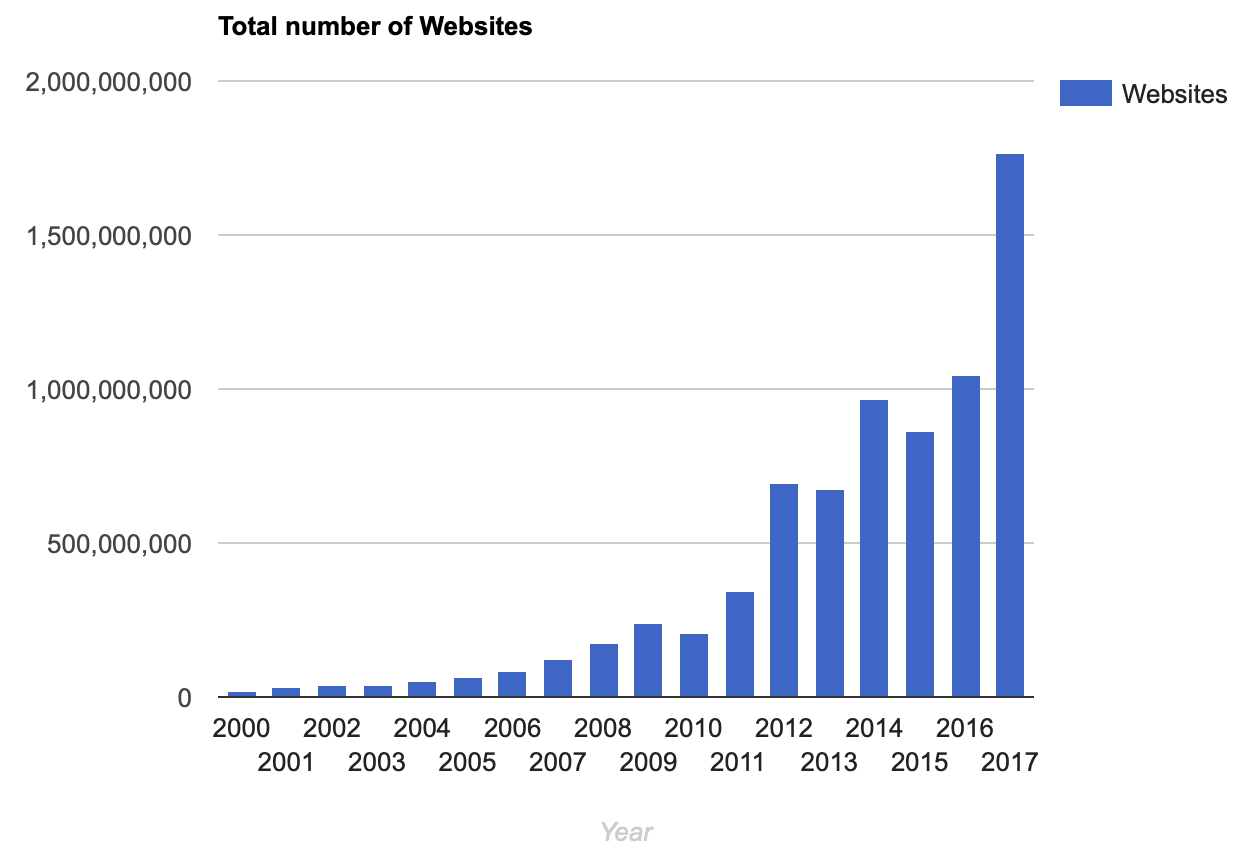
\includegraphics[width=0.5\textwidth]{images/websites}
    \caption{increasing amount of websites ...}
    \label{fig:amountwebsites}
\end{figure}

However, one problem of many state-of-the-art machine learning algorithms is that they can solve one task well, but only this task. Imagine a classifier that can distinguish between different animals. It may have learned to perform very well and can differentiate different animals such as a leopard and a tiger. The classifier learned some certain representations that identify the animals occurately. Nevertheless, the classifier only learned to describe animals. An image such as the one shown in \ref{fig:couch} may be able to trick the classifier by being evaluated as a leopard.

\begin{figure}[h]
    \centering
    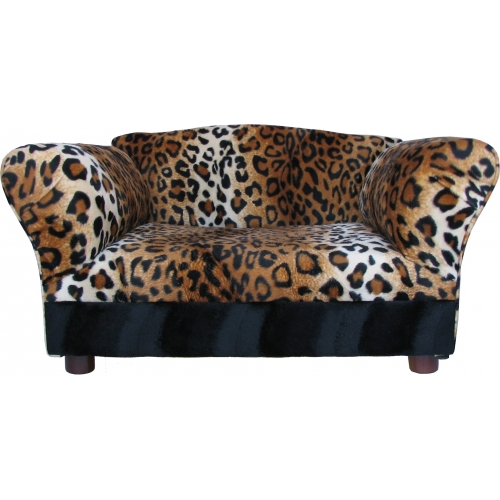
\includegraphics[width=0.5\textwidth]{images/sofa}
    \caption{not a leopard}
    \label{fig:couch}
\end{figure}

Where we can give general information about existing algorithms, their runtime and their accuracy, this thesis aims to design algorithms that are adapted to certain text and image data and thus are able to perform more efficiently on the data than existing general solutions. Also, these algorithms are designed to be adaptable to other clustering tasks within the same data domain.

The here proposed algorithms perform clustering tasks, i.e. they divide existing data into different subspaces. Imagine different animals, one potential subspace could be pets where on the other side there are wild animals. The proposed clustering algoriths belong to a specific family that will be introduced in chapter \ref{chapter:background}.